\documentclass[10pt, aspectratio=169]{beamer}
\usefonttheme{professionalfonts}

\mode<presentation>
{
  \usetheme{Berkeley}
  \usecolortheme{beaver}
  \usefonttheme{default}
  \setbeamertemplate{navigation symbols}{}
  \setbeamertemplate{caption}[numbered]
} 

\setbeamertemplate{footline}{%
  \leavevmode%
  \hbox{%
    \begin{beamercolorbox}[wd=.85\paperwidth,ht=2.5ex,dp=1ex,left]{author in head/foot}%
      \usebeamerfont{author in head/foot}Maxx Seminario, Electronic Circuits, Spring 2026%
    \end{beamercolorbox}%
    \begin{beamercolorbox}[wd=.15\paperwidth,ht=2.5ex,dp=1ex,right]{date in head/foot}%
      \hspace*{0.5em}\insertframenumber{} / \inserttotalframenumber\hspace*{0.5em}%
    \end{beamercolorbox}%
  }%
  \vskip0pt%
}

\usepackage[english]{babel}
\usepackage[utf8x]{inputenc}
\usepackage{tikz}
\usetikzlibrary{shapes.geometric}
\usepackage{pgfplots}
\usepackage{array}
\usepackage{makecell}
\usepackage{verbatim}
\usepackage{graphicx}
\usepackage{subcaption}
\usepackage{amsfonts}
\usepackage{amsmath}
\usepackage{bm}
\usepackage{epstopdf}
\usepackage{circuitikz}
\usepackage{caption}
\usepackage{multirow}
\captionsetup{compatibility=false}
\usepackage[absolute,overlay]{textpos}
\usetikzlibrary{calc}
\usetikzlibrary{pgfplots.fillbetween, backgrounds}
\usetikzlibrary{positioning}
\usetikzlibrary{pgfplots.groupplots}
\usetikzlibrary{plotmarks}
\usetikzlibrary{calc}
\usetikzlibrary{patterns}
\usepgfplotslibrary{groupplots}
\pgfplotsset{compat=newest} 

\usepackage{hyperref}
\definecolor{BeaverRed}{RGB}{179,38,38} 
\hypersetup{
    colorlinks=true,
    linkcolor=BeaverRed,
    filecolor=magenta,      
    urlcolor=cyan,
}

% Added by Maxx Seminario - for colored icons in itemize labels
\usepackage{wasysym} 
\newcommand{\neutralface}{%
  \tikz[baseline=-0.6ex]{
    \draw (0,0) circle (0.9ex);
    \fill (-0.35ex,0.25ex) circle (0.12ex);
    \fill ( 0.35ex,0.25ex) circle (0.12ex);
    \draw (-0.35ex,-0.25ex) -- (0.35ex,-0.25ex);
  }%
}

\newcommand{\baditem}{\textcolor{red! 70! black}{\frownie}}
\newcommand{\gooditem}{\textcolor{green!60!black}{\smiley}}
\newcommand{\mehitem}{\textcolor{orange!80!black}{\neutralface}}

% =========================
% Solution toggle 
% =========================
\newif\ifshowsolutions
\showsolutionstrue   %  compile WITH solutions
%\showsolutionsfalse %  compile WITHOUT solutions

% =========================
% Document Information
% =========================
\title[PN Junction]{The PN Junction}
\subtitle{Formation, Depletion Region, and Built-in Potential}
\author{Maxx Seminario}
\institute{University of Nebraska-Lincoln}
\date{Spring 2026}

\begin{document}

\begin{frame}
  \titlepage
\end{frame}

\section{Introduction}

\begin{frame}{Why Study the PN Junction?}
    
    \begin{columns}[t]
    \column{0.48\textwidth}
        \textbf{Foundation of Semiconductor Devices}: 
        
        \vspace{0.3cm}
        
        \begin{itemize}
            \item Diodes, BJTs, MOSFETs all contain pn junctions
            \item Rectification and switching
            \item Controls current flow
        \end{itemize}
        
        \vspace{0.5cm}
        
        \textbf{Key Questions}:
        \begin{itemize}
            \item What happens when p-type meets n-type? 
            \item How does the depletion region form?
            \item What is built-in potential?
            \item How do carriers move across the junction?
        \end{itemize}
        
    \column{0.48\textwidth}
        \textbf{Applications}:
        \begin{itemize}
            \item Rectifier diodes (AC to DC)
            \item Signal processing
            \item Voltage regulation
            \item Light-emitting diodes (LEDs)
            \item Solar cells
        \end{itemize}
        
        \begin{block}{Lecture Objectives}
            \begin{itemize}
                \item Understand pn junction formation
                \item Analyze depletion region
                \item Calculate built-in potential
                \item Understand drift and diffusion currents
            \end{itemize}
        \end{block}
        
    \end{columns}
    
\end{frame}

\section{Separated Semiconductors}

\begin{frame}{p-Type Semiconductor}
    
    \begin{columns}[t]
    \column{0.48\textwidth}
        \textbf{Carrier Concentrations}:
        \begin{itemize}
            \item Acceptor concentration: $N_A$
            \item Majority carriers (holes): $p \approx N_A$
            \item Minority carriers (electrons): $n \approx \dfrac{n_i^2}{N_A}$
            \item Charge neutral overall
        \end{itemize}
        
        \vspace{0.3cm}
        
        \textbf{Energy Levels}:
        \begin{itemize}
            \item Fermi level $E_F$ near valence band
            \item Many holes in valence band
            \item Few electrons in conduction band
        \end{itemize}
        
    \column{0.48\textwidth}
        \begin{center}
        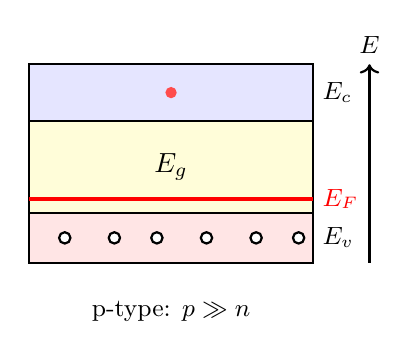
\begin{tikzpicture}[scale=0.9]
            % Energy band diagram
            \draw[thick, fill=blue!10] (0,2.5) rectangle (4,3.3);
            \node[right, font=\small] at (4,2.9) {$E_c$};
            
            \draw[thick, fill=yellow!15] (0,1.2) rectangle (4,2.5);
            \node at (2,1.85) {$E_g$};
            
            % Fermi level
            \draw[very thick, red] (0,1.4) -- (4,1.4);
            \node[right, font=\small, red] at (4,1.4) {$E_F$};
            
            \draw[thick, fill=red!10] (0,0.5) rectangle (4,1.2);
            \node[right, font=\small] at (4,0.85) {$E_v$};
            
            % Few electrons in CB
            \fill[red!70] (2,2.9) circle (0.08cm);
            
            % Many holes in VB
            \foreach \x in {0.5,1.2,1.8,2.5,3.2,3.8} {
                \draw[fill=white, thick] (\x,0.85) circle (0.08cm);
            }
            
            \draw[->, thick] (4.8,0.5) -- (4.8,3.3) node[above, font=\small] {$E$};
            
            \node[below, font=\small] at (2,0.1) {p-type: $p \gg n$};
        \end{tikzpicture}
        \end{center}
        
    \end{columns}
    
\end{frame}

\begin{frame}{n-Type Semiconductor}
    
    \begin{columns}[t]
    \column{0.48\textwidth}
        \textbf{Carrier Concentrations}:
        \begin{itemize}
            \item Donor concentration: $N_D$
            \item Majority carriers (electrons): $n \approx N_D$
            \item Minority carriers (holes): $p \approx \dfrac{n_i^2}{N_D}$
            \item Charge neutral overall
        \end{itemize}
        
        \vspace{0.3cm}
        
        \textbf{Energy Levels}:
        \begin{itemize}
            \item Fermi level $E_F$ near conduction band
            \item Many electrons in conduction band
            \item Few holes in valence band
        \end{itemize}
        
    \column{0.48\textwidth}
        \begin{center}
        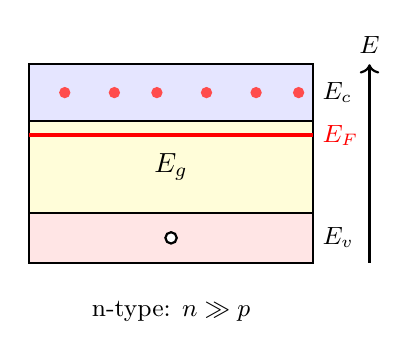
\begin{tikzpicture}[scale=0.9]
            % Energy band diagram
            \draw[thick, fill=blue!10] (0,2.5) rectangle (4,3.3);
            \node[right, font=\small] at (4,2.9) {$E_c$};
            
            \draw[thick, fill=yellow!15] (0,1.2) rectangle (4,2.5);
            \node at (2,1.85) {$E_g$};
            
            % Fermi level
            \draw[very thick, red] (0,2.3) -- (4,2.3);
            \node[right, font=\small, red] at (4,2.3) {$E_F$};
            
            \draw[thick, fill=red!10] (0,0.5) rectangle (4,1.2);
            \node[right, font=\small] at (4,0.85) {$E_v$};
            
            % Many electrons in CB
            \foreach \x in {0.5,1.2,1.8,2.5,3.2,3.8} {
                \fill[red!70] (\x,2.9) circle (0.08cm);
            }
            
            % Few holes in VB
            \draw[fill=white, thick] (2,0.85) circle (0.08cm);
            
            \draw[->, thick] (4.8,0.5) -- (4.8,3.3) node[above, font=\small] {$E$};
            
            \node[below, font=\small] at (2,0.1) {n-type: $n \gg p$};
        \end{tikzpicture}
        \end{center}
        
    \end{columns}
    
\end{frame}

\begin{frame}{Separated p-type and n-type}
    
    \begin{center}
    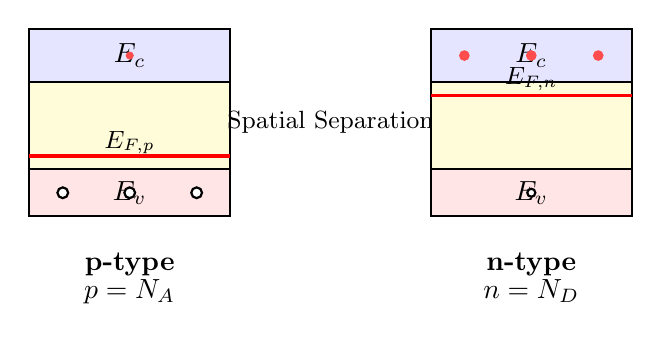
\begin{tikzpicture}[scale=0.85]
        % p-type (left)
        \begin{scope}[xshift=0cm]
            \draw[thick, fill=blue!10] (0,2.5) rectangle (3,3.3);
            \node at (1.5,2.9) {$E_c$};
            
            \draw[thick, fill=yellow!15] (0,1.2) rectangle (3,2.5);
            
            \draw[very thick, red] (0,1.4) -- (3,1.4);
            \node at (1.5,1.6) {\small $E_{F,p}$};
            
            \draw[thick, fill=red!10] (0,0.5) rectangle (3,1.2);
            \node at (1.5,0.85) {$E_v$};
            
            % Holes
            \foreach \x in {0.5,1.5,2.5} {
                \draw[fill=white, thick] (\x,0.85) circle (0.08cm);
            }
            % Few electrons
            \fill[red!70] (1.5,2.9) circle (0.06cm);
            
            \node[below] at (1.5,0.1) {\textbf{p-type}};
            \node[below] at (1.5,-0.3) {$p = N_A$};
        \end{scope}
        
        % Gap
        \node at (4.5,1.9) {\small Spatial Separation};
        
        % n-type (right)
        \begin{scope}[xshift=6cm]
            \draw[thick, fill=blue!10] (0,2.5) rectangle (3,3.3);
            \node at (1.5,2.9) {$E_c$};
            
            \draw[thick, fill=yellow!15] (0,1.2) rectangle (3,2.5);
            
            \draw[very thick, red] (0,2.3) -- (3,2.3);
            \node at (1.5,2.55) {\small $E_{F,n}$};
            
            \draw[thick, fill=red!10] (0,0.5) rectangle (3,1.2);
            \node at (1.5,0.85) {$E_v$};
            
            % Electrons
            \foreach \x in {0.5,1.5,2.5} {
                \fill[red!70] (\x,2.9) circle (0.08cm);
            }
            % Few holes
            \draw[fill=white, thick] (1.5,0.85) circle (0.06cm);
            
            \node[below] at (1.5,0.1) {\textbf{n-type}};
            \node[below] at (1.5,-0.3) {$n = N_D$};
        \end{scope}
        
    \end{tikzpicture}
    \end{center}
    
    \vspace{0.3cm}
    
    \begin{itemize}
        \item \textbf{Different Fermi levels}: $E_{F,p} < E_{F,n}$
        \item \textbf{No current}: Semiconductors are separated
        \item \textbf{What happens when we bring them together?}
    \end{itemize}
    
\end{frame}

\section{Junction Formation}

\begin{frame}{Bringing p-type and n-type Together}
    
    \begin{columns}[t]
    \column{0.48\textwidth}
        \textbf{At $t = 0^+$ (instant of contact)}:
        \begin{itemize}
            \item Large concentration gradients exist
            \item Electrons in n-side: high concentration
            \item Holes in p-side: high concentration
            \item \textbf{Diffusion begins}
        \end{itemize}
        
        \vspace{0.3cm}
        
        \textbf{Diffusion Process}:
        \begin{itemize}
            \item Electrons diffuse from n $\rightarrow$ p
            \item Holes diffuse from p $\rightarrow$ n
            \item Leaves behind ionized dopants
            \item Creates space charge region
        \end{itemize}
        
    \column{0.48\textwidth}
        \begin{center}
        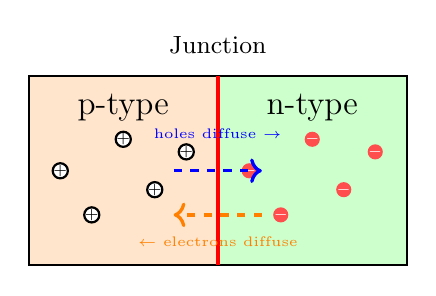
\begin{tikzpicture}[scale=0.8]
            % p-type region
            \draw[thick, fill=orange!20] (0,0) rectangle (3,3);
            \node[font=\large] at (1.5,2.5) {p-type};
            
            % Holes (positive charges)
            \foreach \x/\y in {0.5/1.5, 1.0/0.8, 1.5/2.0, 2.0/1.2, 2.5/1.8} {
                \draw[fill=white, thick] (\x,\y) circle (0.12cm) node[black, font=\tiny] {$+$};
            }
            
            % n-type region
            \draw[thick, fill=green!20] (3,0) rectangle (6,3);
            \node[font=\large] at (4.5,2.5) {n-type};
            
            % Electrons (negative charges)
            \foreach \x/\y in {3.5/1.5, 4.0/0.8, 4.5/2.0, 5.0/1.2, 5.5/1.8} {
                \fill[red!70] (\x,\y) circle (0.12cm);
                \node[white, font=\tiny] at (\x,\y) {$-$};
            }
            
            % Junction line
            \draw[ultra thick, red] (3,0) -- (3,3);
            \node[above, font=\small] at (3,3.2) {Junction};
            
            % Diffusion arrows
            \draw[->, very thick, blue, dashed] (2.3,1.5) -- (3.7,1.5);
            \node[above, font=\tiny, blue] at (3,1.85) {holes diffuse $\rightarrow$};
            
            \draw[->, very thick, orange, dashed] (3.7,0.8) -- (2.3,0.8);
            \node[below, font=\tiny, orange] at (3,0.6) {$\leftarrow$ electrons diffuse};
            
        \end{tikzpicture}
        \end{center}
        
    \end{columns}
    
\end{frame}

\begin{frame}{Formation of Depletion Region}
    
    \begin{center}
    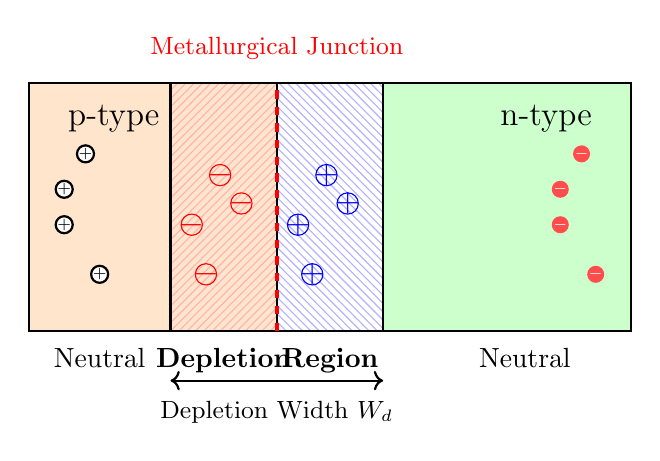
\begin{tikzpicture}[scale=0.9]
        % p-type region
        \draw[thick, fill=orange!20] (0,0) rectangle (3.5,3.5);
        \node[font=\large] at (1.2,3) {p-type};
        
        % Neutral p-region with holes
        \foreach \x/\y in {0.5/1.5, 0.8/2.5, 1.0/0.8, 0.5/2.0} {
            \draw[fill=white, thick] (\x,\y) circle (0.12cm) node[black, font=\tiny] {$+$};
        }
        
        % Depletion region on p-side
        \draw[thick, fill=red!15, pattern=north east lines, pattern color=red!30] (2.0,0) rectangle (3.5,3.5);
        % Negative acceptor ions
        \foreach \x/\y in {2.3/1.5, 2.7/2.2, 2.5/0.8, 3.0/1.8} {
            \node[red, font=\large] at (\x,\y) {$-$};
            \draw[red] (\x,\y) circle (0.15cm);
        }
        
        % Depletion region on n-side
        \draw[thick, fill=blue!15, pattern=north west lines, pattern color=blue!30] (3.5,0) rectangle (5.0,3.5);
        % Positive donor ions
        \foreach \x/\y in {3.8/1.5, 4.2/2.2, 4.0/0.8, 4.5/1.8} {
            \node[blue, font=\large] at (\x,\y) {$+$};
            \draw[blue] (\x,\y) circle (0.15cm);
        }
        
        % n-type region
        \draw[thick, fill=green!20] (5.0,0) rectangle (8.5,3.5);
        \node[font=\large] at (7.3,3) {n-type};
        
        % Neutral n-region with electrons
        \foreach \x/\y in {7.5/1.5, 7.8/2.5, 8.0/0.8, 7.5/2.0} {
            \fill[red!70] (\x,\y) circle (0.12cm);
            \node[white, font=\tiny] at (\x,\y) {$-$};
        }
        
        % Labels
        \node[below] at (1.0,-0.1) {Neutral};
        \node[below] at (2.75,-0.1) {\textbf{Depletion}};
        \node[below] at (4.25,-0.1) {\textbf{Region}};
        \node[below] at (7.0,-0.1) {Neutral};
        
        \draw[<->, thick] (2.0,-0.7) -- (5.0,-0.7);
        \node[below, font=\small] at (3.5,-0.85) {Depletion Width $W_d$};
        
        % Junction line
        \draw[ultra thick, red, dashed] (3.5,0) -- (3.5,3.5);
        \node[above, font=\small, red] at (3.5,3.7) {Metallurgical Junction};
        
    \end{tikzpicture}
    \end{center}
    
    \begin{itemize}
        \item \textbf{Depletion region}: Region depleted of mobile carriers (electrons and holes)
        \item \textbf{Space charge}: Fixed ionized dopant atoms create electric field
        \item \textbf{Self-limiting process}: Electric field opposes further diffusion
    \end{itemize}
    
\end{frame}

\begin{frame}{Charge Distribution at Junction}
    
    \begin{center}
    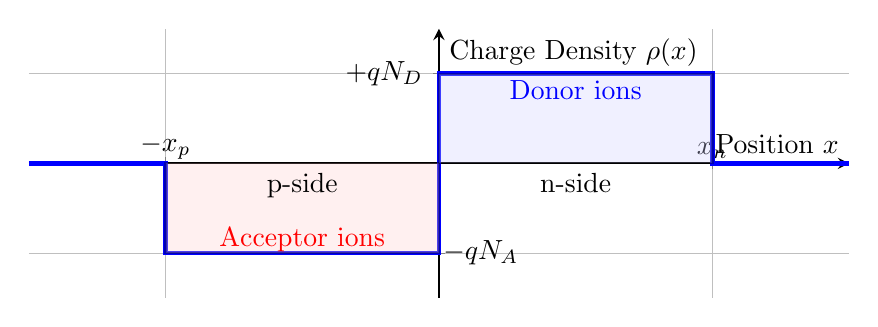
\begin{tikzpicture}[scale=1.0]
        \begin{axis}[
            width=12cm, height=5cm,
            xlabel={Position $x$},
            ylabel={Charge Density $\rho(x)$},
            ylabel style={at={(axis description cs:0,1.02)}, anchor=south},
            xmin=-3, xmax=3,
            ymin=-1.5, ymax=1.5,
            xtick={-2, 0, 2},
            xticklabels={$-x_p$, $0$, $x_n$},
            xticklabel style={anchor=south},
            ytick={0, 1},
            yticklabels={$0$, $+qN_D$},
            extra y ticks={-1},
            extra y tick labels={$-qN_A$},
            extra y tick style={yticklabel style={anchor=west}},
            grid=major,
            axis lines=middle,
            samples=100,
            domain=-3:3,
            thick,
        ]
        
        % Charge density - rectangular approximation
        \addplot[blue, ultra thick] coordinates {
            (-3, 0)
            (-2, 0)
            (-2, -1)
            (0, -1)
            (0, 1)
            (2, 1)
            (2, 0)
            (3, 0)
        };
        
        % Shaded regions
        \addplot[fill=red!20, opacity=0.3] coordinates {
            (-2, 0) (-2, -1) (0, -1) (0, 0)
        } -- cycle;
        
        \addplot[fill=blue!20, opacity=0.3] coordinates {
            (0, 0) (0, 1) (2, 1) (2, 0)
        } -- cycle;
        
        % Labels
        \node[anchor=north] at (axis cs:-1,0) {p-side};
        \node[anchor=north] at (axis cs:1,0) {n-side};
        \node[anchor=south, red] at (axis cs:-1,-1.1) {Acceptor ions};
        \node[anchor=south, blue] at (axis cs:1,0.6) {Donor ions};
        
        \end{axis}
    \end{tikzpicture}
    \end{center}
    
    \vspace{0.2cm}
    
    \begin{itemize}
        \item \textbf{p-side depletion}: Negatively charged acceptor ions ($-qN_A$)
        \item \textbf{n-side depletion}: Positively charged donor ions ($+qN_D$)
        \item \textbf{Charge neutrality}: $qN_A x_p = qN_D x_n$ (total charge = 0)
    \end{itemize}
    
\end{frame}

\begin{frame}{Electric Field in Depletion Region}
    
    \begin{center}
    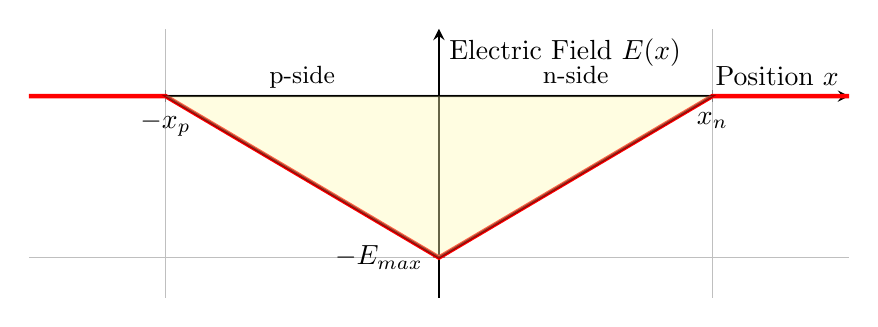
\begin{tikzpicture}[scale=1.0]
        \begin{axis}[
            width=12cm, height=5cm,
            xlabel={Position $x$},
            ylabel={Electric Field $E(x)$},
            xmin=-3, xmax=3,
            ymin=-1.5, ymax=0.5,
            xtick={-2, 0, 2},
            xticklabels={$-x_p$, $0$, $x_n$},
            ytick={-1.2, 0},
            yticklabels={$-E_{max}$, $0$},
            grid=major,
            axis lines=middle,
            samples=100,
            thick,
        ]
        
        % Electric field - triangular shape
        \addplot[red, ultra thick] coordinates {
            (-3, 0)
            (-2, 0)
            (0, -1.2)
            (2, 0)
            (3, 0)
        };
        
        % Shaded region
        \addplot[fill=yellow!30, opacity=0.4] coordinates {
            (-2, 0) (0, -1.2) (2, 0)
        } -- cycle;
        
        % Labels
        \node[anchor=north, font=\small] at (axis cs:-1,0.3) {p-side};
        \node[anchor=north, font=\small] at (axis cs:1,0.3) {n-side};
        
        \end{axis}
    \end{tikzpicture}
    \end{center}
    
    \vspace{0.2cm}
    
    \begin{itemize}
        \item \textbf{Direction}: Electric field points from n-side to p-side (from + to -)
        \item \textbf{Maximum at junction}: $E_{max}$ occurs at metallurgical junction
        \item \textbf{Creates built-in potential}: $V_{bi} = -\int E(x) dx$
    \end{itemize}
    
\end{frame}

\begin{frame}{Built-in Potential}
    
    \begin{center}
    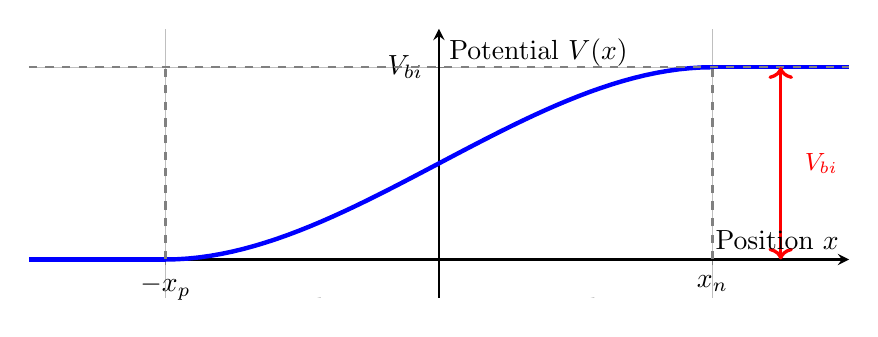
\begin{tikzpicture}[scale=1.0]
        \begin{axis}[
            width=12cm, height=5cm,
            xlabel={Position $x$},
            ylabel={Potential $V(x)$},
            xmin=-3, xmax=3,
            ymin=-0.2, ymax=1.2,
            xtick={-2, 0, 2},
            xticklabels={$-x_p$, $0$, $x_n$},
            ytick={0, 1},
            yticklabels={$0$, $V_{bi}$},
            grid=major,
            axis lines=middle,
            samples=100,
            thick,
        ]
        
        % Potential - smooth sigmoid-like curve from p-side (0V) to n-side (V_bi)
        \addplot[blue, ultra thick] coordinates {(-3, 0) (-2, 0)};
        \addplot[blue, ultra thick, domain=-2:2, samples=50] {3*((x+2)/4)^2 - 2*((x+2)/4)^3};
        \addplot[blue, ultra thick] coordinates {(2, 1) (3, 1)};
        
        % Dashed lines
        \draw[dashed, gray] (axis cs:-2,0) -- (axis cs:-2,1);
        \draw[dashed, gray] (axis cs:2,0) -- (axis cs:2,1);
        \draw[dashed, gray] (axis cs:-3,1) -- (axis cs:3,1);
        
        % Arrow showing V_bi
        \draw[<->, very thick, red] (axis cs:2.5,0) -- (axis cs:2.5,1);
        \node[right, font=\small, red] at (axis cs:2.6,0.5) {$V_{bi}$};
        
        % Labels
        \node[anchor=north, font=\small] at (axis cs:-1,-0.15) {p-side};
        \node[anchor=north, font=\small] at (axis cs:1,-0.15) {n-side};
        
        \end{axis}
    \end{tikzpicture}
    \end{center}
    
    \vspace{0.2cm}
    
    \begin{block}{Built-in Potential Formula}
        $$V_{bi} = \frac{kT}{q} \ln\left(\frac{N_A N_D}{n_i^2}\right) = V_T \ln\left(\frac{N_A N_D}{n_i^2}\right)$$
        where $V_T = \frac{kT}{q} \approx 26$ mV at room temperature (300 K)
    \end{block}
    
\end{frame}

\section{Thermal Equilibrium}

\begin{frame}{Energy Band Diagram at Thermal Equilibrium}
    
    \begin{center}
    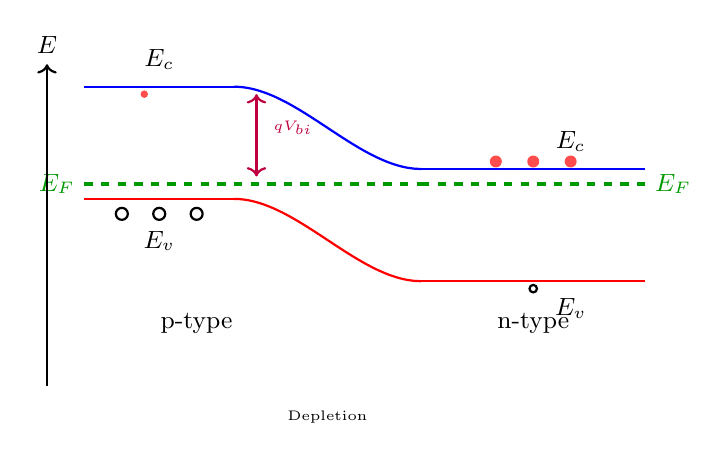
\begin{tikzpicture}[scale=0.95]
        % p-type region (x: 0 to 2, Ec at 3, Ev at 1.5)
        \begin{scope}[xshift=0cm]
            % Conduction band - flat in p-region
            \draw[thick, blue] (0,3) -- (2,3);
            \node[above, font=\small] at (1,3.1) {$E_c$};
            
            % Valence band - flat in p-region
            \draw[thick, red] (0,1.5) -- (2,1.5);
            \node[below, font=\small] at (1,1.2) {$E_v$};
            
            % Fermi level (flat at equilibrium)
            \draw[very thick, green!60!black, dashed] (0,1.7) -- (2,1.7);
            \node[left, font=\small, green!60!black] at (0,1.7) {$E_F$};
            
            % Holes in p-region
            \foreach \x in {0.5,1.0,1.5} {
                \draw[fill=white, thick] (\x,1.3) circle (0.08cm);
            }
            
            % Few electrons in p-region
            \fill[red!70] (0.8,2.9) circle (0.05cm);
            
            \node[below, font=\small] at (1.5,0.1) {p-type};
        \end{scope}
        
        \begin{scope}[xshift=0cm]
            % Conduction band sigmoid: y = 3 - 1.1*(3t^2 - 2t^3) where t = (x-2)/2.5
            \draw[thick, blue, domain=2:4.5, samples=30, smooth] 
                plot (\x, {3 - 1.1*(3*(((\x-2)/2.5)^2) - 2*(((\x-2)/2.5)^3))});
            
            % Valence band sigmoid: y = 1.5 - 1.1*(3t^2 - 2t^3) where t = (x-2)/2.5
            \draw[thick, red, domain=2:4.5, samples=30, smooth] 
                plot (\x, {1.5 - 1.1*(3*(((\x-2)/2.5)^2) - 2*(((\x-2)/2.5)^3))});
            
            % Fermi level continues flat
            \draw[very thick, green!60!black, dashed] (2,1.7) -- (4.5,1.7);
            
            \node[below, font=\tiny] at (3.25,-1.2) {Depletion};
            
            % Draw potential barrier
            \draw[<->, thick, purple] (2.3,1.8) -- (2.3,2.9);
            \node[right, font=\tiny, purple] at (2.4,2.45) {$qV_{bi}$};
        \end{scope}
        
        % n-type region (x: 4.5 to 7.5, Ec at 1.9, Ev at 0.4)
        \begin{scope}[xshift=0cm]
            % Conduction band - flat in n-region
            \draw[thick, blue] (4.5,1.9) -- (7.5,1.9);
            \node[above, font=\small] at (6.5,2.0) {$E_c$};
            
            % Valence band - flat in n-region
            \draw[thick, red] (4.5,0.4) -- (7.5,0.4);
            \node[below, font=\small] at (6.5,0.3) {$E_v$};
            
            % Fermi level
            \draw[very thick, green!60!black, dashed] (4.5,1.7) -- (7.5,1.7);
            \node[right, font=\small, green!60!black] at (7.5,1.7) {$E_F$};
            
            % Electrons in n-region
            \foreach \x in {5.5,6.0,6.5} {
                \fill[red!70] (\x,2.0) circle (0.08cm);
            }
            
            % Few holes in n-region
            \draw[fill=white, thick] (6.0,0.3) circle (0.05cm);
            
            \node[below, font=\small] at (6.0,0.1) {n-type};
        \end{scope}
        
        % Energy axis
        \draw[->, thick] (-0.5,-1) -- (-0.5,3.3) node[above, font=\small] {$E$};
        
    \end{tikzpicture}
    \end{center}
    
    \begin{itemize}
        \item \textbf{Fermi level is flat}: At thermal equilibrium, $E_F$ is constant throughout
        \item \textbf{Band bending}: Energy bands bend by $qV_{bi}$ across depletion region
        \item \textbf{Barrier for electrons and holes}: Prevents unlimited diffusion
    \end{itemize}
    
\end{frame}

\begin{frame}{Drift and Diffusion Currents at Equilibrium}
    
    \begin{center}
    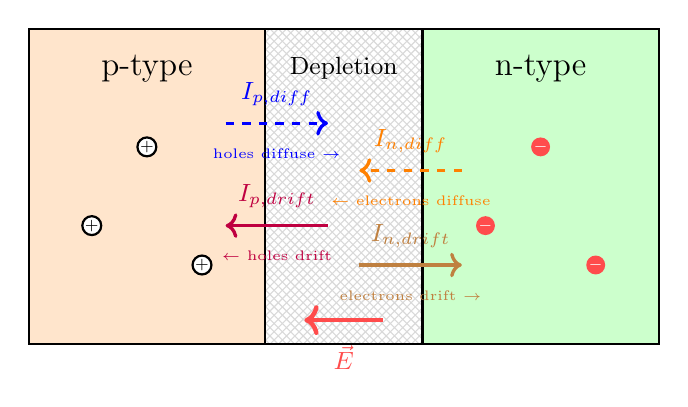
\begin{tikzpicture}[scale=1.0]
        % p-type region
        \draw[thick, fill=orange!20] (0,0) rectangle (3,4);
        \node[font=\large] at (1.5,3.5) {p-type};
        
        % Depletion region
        \draw[thick, fill=yellow!30, pattern=crosshatch, pattern color=gray!30] (3,0) rectangle (5,4);
        \node[font=\small] at (4,3.5) {Depletion};
        
        % n-type region
        \draw[thick, fill=green!20] (5,0) rectangle (8,4);
        \node[font=\large] at (6.5,3.5) {n-type};
        
        % Holes in p-region
        \foreach \x/\y in {0.8/1.5, 1.5/2.5, 2.2/1.0} {
            \draw[fill=white, thick] (\x,\y) circle (0.12cm) node[black, font=\tiny] {$+$};
        }
        
        % Electrons in n-region
        \foreach \x/\y in {5.8/1.5, 6.5/2.5, 7.2/1.0} {
            \fill[red!70] (\x,\y) circle (0.12cm);
            \node[white, font=\tiny] at (\x,\y) {$-$};
        }
        
        % Diffusion currents (from high to low concentration)
        \draw[->, very thick, blue, dashed] (2.5,2.8) -- (3.8,2.8);
        \node[above, font=\small, blue] at (3.15,2.9) {$I_{p,diff}$};
        \node[below, font=\tiny, blue] at (3.15,2.6) {holes diffuse $\rightarrow$};
        
        \draw[->, very thick, orange, dashed] (5.5,2.2) -- (4.2,2.2);
        \node[above, font=\small, orange] at (4.85,2.3) {$I_{n,diff}$};
        \node[below, font=\tiny, orange] at (4.85,2.0) {$\leftarrow$ electrons diffuse};
        
        % Drift currents (due to electric field)
        \draw[->, very thick, purple] (3.8,1.5) -- (2.5,1.5);
        \node[above, font=\small, purple] at (3.15,1.6) {$I_{p,drift}$};
        \node[below, font=\tiny, purple] at (3.15,1.3) {$\leftarrow$ holes drift};
        
        \draw[->, very thick, brown] (4.2,1.0) -- (5.5,1.0);
        \node[above, font=\small, brown] at (4.85,1.1) {$I_{n,drift}$};
        \node[below, font=\tiny, brown] at (4.85,0.8) {electrons drift $\rightarrow$};
        
        % Electric field arrow
        \draw[->, ultra thick, red!70] (4.5,0.3) -- (3.5,0.3);
        \node[below, font=\small, red!70] at (4,0.1) {$\vec{E}$};
        
    \end{tikzpicture}
    \end{center}
    
    \begin{block}{At Thermal Equilibrium}
        \begin{itemize}
            \item $I_{p,diff} + I_{p,drift} = 0$ (hole current = 0)
            \item $I_{n,diff} + I_{n,drift} = 0$ (electron current = 0)
            \item Total current $I = 0$
        \end{itemize}
    \end{block}
    
\end{frame}

\begin{frame}{Concentration Profiles}
    
    \begin{columns}[t]
    \column{0.48\textwidth}
        \textbf{Hole Concentration $p(x)$}:
        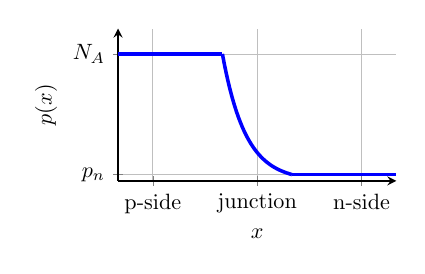
\begin{tikzpicture}[scale=0.8]
        \begin{axis}[
            width=6cm, height=4cm,
            xlabel={$x$},
            ylabel={$p(x)$},
            xmin=-2, xmax=2,
            ymin=0, ymax=1.2,
            xtick={-1.5, 0, 1.5},
            xticklabels={p-side, junction, n-side},
            ytick={0.05, 1},
            yticklabels={$p_n$, $N_A$},
            grid=major,
            axis lines=left,
            thick,
        ]
        
        % Hole concentration
        \addplot[blue, ultra thick, domain=-2:-0.5] {1};
        \addplot[blue, ultra thick, domain=-0.5:0.5, samples=40] {exp(-2.996*(x+0.5))};
        \addplot[blue, ultra thick, domain=0.5:2] {0.05};
        
        \end{axis}
        \end{tikzpicture}
        
        \begin{itemize}
            \item High on p-side ($p \approx N_A$)
            \item Low on n-side ($p \approx \frac{n_i^2}{N_D}$)
            \item Exponential in depletion region
        \end{itemize}
    
    \column{0.48\textwidth}
        \textbf{Electron Concentration $n(x)$}:
        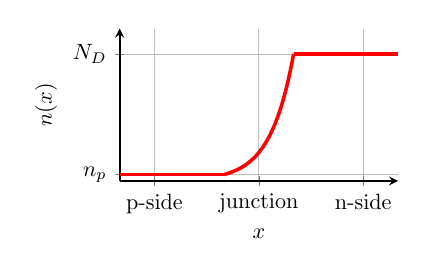
\begin{tikzpicture}[scale=0.8]
        \begin{axis}[
            width=6cm, height=4cm,
            xlabel={$x$},
            ylabel={$n(x)$},
            xmin=-2, xmax=2,
            ymin=0, ymax=1.2,
            xtick={-1.5, 0, 1.5},
            xticklabels={p-side, junction, n-side},
            ytick={0.05, 1},
            yticklabels={$n_p$, $N_D$},
            grid=major,
            axis lines=left,
            thick,
        ]
        
        % Electron concentration
        \addplot[red, ultra thick, domain=-2:-0.5] {0.05};
        \addplot[red, ultra thick, domain=-0.5:0.5, samples=40] {0.05*exp(2.996*(x+0.5))};
        \addplot[red, ultra thick, domain=0.5:2] {1};
        
        \end{axis}
        \end{tikzpicture}
        
        \begin{itemize}
            \item Low on p-side ($n \approx \frac{n_i^2}{N_A}$)
            \item High on n-side ($n \approx N_D$)
            \item Exponential in depletion region
        \end{itemize}
    
    \end{columns}
    
\end{frame}

\section{Summary}

\begin{frame}{Key Formulas Reference}
    
    \begin{columns}[T]
    \column{0.48\textwidth}
    \begin{table}[t]
    \centering
    \renewcommand{\arraystretch}{1.8}
    \small
    \begin{tabular}{|l|c|}
    \hline
    \textbf{Parameter} & \textbf{Formula} \\
    \hline
    \hline
    Built-in potential & $V_{bi} = V_T \ln\left(\dfrac{N_A N_D}{n_i^2}\right)$ \\
    \hline
    Thermal voltage & $V_T = \dfrac{kT}{q} \approx 26$ mV \\
    \hline
    Depletion width & $W = x_p + x_n$ \\
    \hline
    Charge neutrality & $N_A x_p = N_D x_n$ \\
    \hline
    \end{tabular}
    \end{table}
    
    \column{0.48\textwidth}
    \begin{table}[t]
    \centering
    \renewcommand{\arraystretch}{1.8}
    \small
    \begin{tabular}{|l|c|}
    \hline
    \textbf{Parameter} & \textbf{Formula} \\
    \hline
    \hline
    Max electric field & $E_{max} = \dfrac{qN_D x_n}{\epsilon_s}$ \\
    \hline
    Equilibrium condition & $I_{diff} + I_{drift} = 0$ \\
    \hline
    Minority carriers (p-side) & $n_p = \dfrac{n_i^2}{N_A}$ \\
    \hline
    Minority carriers (n-side) & $p_n = \dfrac{n_i^2}{N_D}$ \\
    \hline
    \end{tabular}
    \end{table}
    \end{columns}
    
\end{frame}

\begin{frame}{Summary: PN Junction Fundamentals}
    
    \begin{enumerate}
        \item \textbf{Junction Formation}:
        \begin{itemize}
            \item Diffusion of carriers creates depletion region
            \item Space charge creates electric field
            \item Built-in potential opposes further diffusion
        \end{itemize}
        
        \item \textbf{Depletion Region}:
        \begin{itemize}
            \item Depleted of mobile carriers
            \item Contains fixed ionized dopants
            \item Width depends on doping concentrations
        \end{itemize}
        
        \item \textbf{Thermal Equilibrium}:
        \begin{itemize}
            \item Fermi level is flat throughout device
            \item Energy bands bend by $qV_{bi}$
            \item Diffusion and drift currents balance (total current = 0)
        \end{itemize}
        
        \item \textbf{Key Concepts}:
        \begin{itemize}
            \item Built-in potential $V_{bi}$ cannot be measured externally
            \item Barrier prevents majority carrier flow
            \item Foundation for understanding diode operation under bias
        \end{itemize}
    \end{enumerate}
    
\end{frame}

\end{document}
